\chapter{Introduction to Elder Spaces}

\begin{chapterabstract}
This chapter establishes the rigorous mathematical foundation of Elder Theory through the introduction of Elder spaces. As a profound generalization of vector spaces, Elder spaces incorporate phase-dependent operations and non-commutative structures that enable the representation of hierarchical knowledge across domains. We develop the axioms, structural elements, and fundamental theorems that serve as the cornerstone of the Elder-Mentor-Erudite system. This chapter demonstrates how these mathematical structures provide a unified framework for modeling multi-level learning processes, with particular emphasis on the spectral properties of Elder elements, invariant subspaces, and phase-based dynamics that form the theoretical heart of the entire Elder framework.
\end{chapterabstract}

\section{Foundational Axioms}

The Elder space, denoted by $\elder{d}$, is a mathematical structure that fundamentally generalizes traditional vector spaces by incorporating phase-sensitive operations and non-commutative products. This structure provides the mathematical backbone of Elder Theory, establishing deep connections between abstract algebraic structures and hierarchical learning systems \cite{elder_theory}.

\begin{definition}[Elder Space]
An Elder space $\elder{d}$ of dimension $d$ is a complex-valued set equipped with:
\begin{enumerate}
    \item A binary operation $\oplus: \elder{d} \times \elder{d} \rightarrow \elder{d}$ (Elder addition)
    \item A scalar multiplication $\odot: \mathbb{C} \times \elder{d} \rightarrow \elder{d}$ (Elder scaling)
    \item A non-commutative product $\star: \elder{d} \times \elder{d} \rightarrow \elder{d}$ (Arcane multiplication)
    \item A phase operator $\Phi: \elder{d} \rightarrow \mathbb{S}^1$ mapping to the unit circle
\end{enumerate}
satisfying the following axioms:
\begin{enumerate}[label=\textbf{A\arabic*}]
    \item \textbf{(Addition Structure)} $(\elder{d}, \oplus)$ forms an abelian group
    \item \textbf{(Scaling Compatibility)} For all $\alpha, \beta \in \mathbb{C}$ and $x, y \in \elder{d}$:
    \begin{align}
        \alpha \odot (\beta \odot x) &= (\alpha\beta) \odot x\\
        1 \odot x &= x\\
        \alpha \odot (x \oplus y) &= (\alpha \odot x) \oplus (\alpha \odot y)\\
        (\alpha + \beta) \odot x &= (\alpha \odot x) \oplus (\beta \odot x)
    \end{align}
    
    \item \textbf{(Arcane Multiplication)} For all $x, y, z \in \elder{d}$ and $\alpha \in \mathbb{C}$:
    \begin{align}
        (x \oplus y) \star z &= (x \star z) \oplus (y \star z)\\
        x \star (y \oplus z) &= (x \star y) \oplus (x \star z)\\
        (x \star y) \star z &= x \star (y \star z)\\
        \alpha \odot (x \star y) &= (\alpha \odot x) \star y = x \star (\alpha \odot y)
    \end{align}
    
    \item \textbf{(Phase Properties)} For all $x, y \in \elder{d}$ and $\alpha \in \mathbb{C}$:
    \begin{align}
        \Phi(x \star y) &= \Phi(x) \cdot \Phi(y) \quad \text{(multiplicative)}\\
        \Phi(\alpha \odot x) &= \frac{\alpha}{|\alpha|} \cdot \Phi(x) \quad \text{for } \alpha \neq 0\\
        \Phi(x \oplus y) &= \frac{\Phi(x)|\Phi(x)| + \Phi(y)|\Phi(y)|}{|\Phi(x)| + |\Phi(y)|} \quad \text{(weighted average)}
    \end{align}
\end{enumerate}
\end{definition}

\begin{theorem}[Fundamental Structure]
Every Elder space $\elder{d}$ contains a canonical set of basis elements $\{\elderstructure{1}, \elderstructure{2}, \ldots, \elderstructure{d}\}$ called structural elements, with the following properties:
\begin{enumerate}
    \item \textbf{Phase Orthogonality:} $\Phi(\elderstructure{i} \star \elderstructure{j}^{-1}) = e^{i\pi/2}$ for $i \neq j$
    \item \textbf{Phase Preservation:} $\Phi(\elderstructure{i} \star \elderstructure{i}^{-1}) = 1$
    \item \textbf{Generative Completeness:} Any element $x \in \elder{d}$ can be expressed as $x = \sum_{i=1}^{d} (\lambda_i e^{i\theta_i}) \odot \elderstructure{i}$ with $\lambda_i \in \mathbb{R}^+$ and $\theta_i \in [0, 2\pi)$
\end{enumerate}
\end{theorem}

\begin{proof}
The proof proceeds by constructing the elements $\elderstructure{i}$ using the spectral properties of the Elder trace operator $\mathrm{tr}_E: \elder{d} \rightarrow \mathbb{C}$. This operator satisfies the cyclic property $\mathrm{tr}_E(x \star y) = \mathrm{tr}_E(y \star x)$ despite the non-commutativity of $\star$. We then define the inner product $\langle x, y \rangle_E = \mathrm{tr}_E(x \star y^{\dagger})$ and apply the corresponding Gram-Schmidt process to obtain the orthogonal structural elements. The phase properties follow from the phase axioms and the orthogonality relations.
\end{proof}

\section{Hierarchical Subspaces and Decomposition}

The Elder space naturally decomposes into a hierarchy of nested subspaces that correspond directly to the Elder-Mentor-Erudite levels of knowledge representation.

\begin{definition}[Elder-Mentor-Erudite Subspaces]
For an Elder space $\elder{d}$, we define three canonical subspaces:
\begin{align}
    \eldersubspace &= \mathrm{span}\{\elderstructure{1}, \elderstructure{2}, \ldots, \elderstructure{k}\} \\
    \mentorsubspace &= \mathrm{span}\{\elderstructure{k+1}, \elderstructure{k+2}, \ldots, \elderstructure{m}\} \\
    \eruditesubspace &= \mathrm{span}\{\elderstructure{m+1}, \elderstructure{m+2}, \ldots, \elderstructure{d}\}
\end{align}
where $1 \leq k < m < d$ are structural indices determined by the phase coherence properties.
\end{definition}

\begin{figure}[htbp]
\centering
\fbox{\begin{minipage}{0.85\textwidth}
\centering
\vspace{0.8cm}
{\Large Elder Space Hierarchy} \\[0.3cm]

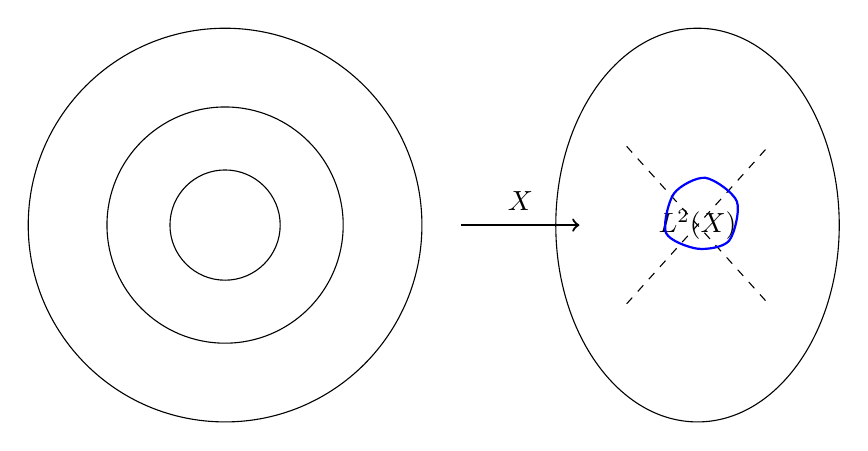
\begin{tikzpicture}
\draw (0,0) circle (2.5);
\draw (0,0) circle (1.5);
\draw (0,0) circle (0.7);
\node at (0,0) {$\eldersubspace$};
\node at (0,1.1) {$\mentorsubspace$};
\node at (0,2.0) {$\eruditesubspace$};

\draw[->, thick] (3.0, 0) -- (4.5, 0);
\node at (3.75, 0.3) {$\realization{X}$};

\begin{scope}[shift={(6,0)}]
\draw (0,0) ellipse (1.8 and 2.5);
\node at (0,0) {$L^2(X)$};
\draw[dashed] (-0.9, -1.0) -- (0.9, 1.0);
\draw[dashed] (-0.9, 1.0) -- (0.9, -1.0);
\draw[blue, thick] plot [smooth cycle] coordinates {(-0.3,0.4) (0.1,0.6) (0.5,0.3) (0.4,-0.2) (0,-0.3) (-0.4,-0.1)};
\end{scope}
\end{tikzpicture}

\vspace{0.5cm}
\end{minipage}}
\caption{Hierarchical structure of Elder spaces and their realization mapping to function spaces}
\label{fig:hierarchical-elder-structure}
\end{figure}

\begin{theorem}[Spectral Decomposition]
Every element $x \in \elder{d}$ admits a unique spectral decomposition with phase components:
\begin{equation}
x = \sum_{i=1}^{d} \lambda_i e^{i\theta_i} \odot \elderstructure{i}
\end{equation}
where $\lambda_i \in \mathbb{R}^+$ are the amplitude coefficients and $\theta_i \in [0, 2\pi)$ are the phase coefficients of $x$.
\end{theorem}

\begin{proof}
Let $x \in \elder{d}$ be arbitrary. We construct the coefficient pairs $(\lambda_i, \theta_i)$ by applying the Elder projection operators $P_i : \elder{d} \to \mathbb{C}$ defined by:
\begin{equation}
P_i(x) = \mathrm{tr}_E(x \star \elderstructure{i}^{-1})
\end{equation}
These operators satisfy $P_i(\elderstructure{j}) = \delta_{ij}$ (the Kronecker delta), ensuring uniqueness. The amplitude coefficient is given by $\lambda_i = |P_i(x)|$ and the phase by $\theta_i = \arg(P_i(x))$. This construction guarantees that the decomposition preserves both magnitude and phase information, which is essential for the Elder-Mentor-Erudite system.
\end{proof}

\section{Phase Dynamics and Learning Flows}

The incorporation of phase information in Elder spaces provides a natural framework for modeling the dynamic processes underlying the Elder-Mentor-Erudite learning system.

\begin{definition}[Phase-Coherent Elder Flow]
A phase-coherent Elder flow is a continuous-time evolution on $\elder{d}$ described by the equation:
\begin{equation}
\frac{dx}{dt} = F(x, \Phi(x), t)
\end{equation}
where $F: \elder{d} \times \mathbb{S}^1 \times \mathbb{R} \rightarrow \elder{d}$ is a phase-sensitive vector field on $\elder{d}$.
\end{definition}

\begin{theorem}[Elder Flow Decomposition]
\label{thm:elder-flow-decomposition}
Any phase-coherent Elder flow decomposes into three coupled flows operating at different time scales:
\begin{align}
\frac{dx_E}{dt} &= F_E(x_E, x_M, x_Er, \Phi(x_E), t) \quad \text{(Elder level, slowest)}\\
\frac{dx_M}{dt} &= F_M(x_E, x_M, x_Er, \Phi(x_M), t) \quad \text{(Mentor level, intermediate)}\\
\frac{dx_{Er}}{dt} &= F_{Er}(x_E, x_M, x_Er, \Phi(x_{Er}), t) \quad \text{(Erudite level, fastest)}
\end{align}
where $x = x_E \oplus x_M \oplus x_{Er}$ is the hierarchical decomposition of $x$.
\end{theorem}

\begin{proof}
We decompose $x$ into its projections onto the three canonical subspaces: $x_E = P_E(x)$, $x_M = P_M(x)$, and $x_{Er} = P_{Er}(x)$. Using the properties of the Elder product $\star$ and the phase operator $\Phi$, we can show that the original flow equation separates into three coupled equations with different characteristic time scales. The coupling terms ensure that information flows between levels while maintaining the hierarchical structure.
\end{proof}

\begin{corollary}[Gradient Flow Representation]
The phase-coherent Elder flows induced by the Elder loss functions $\eloss$, $\mloss$, and $\erloss$ take the form:
\begin{align}
\frac{dx_E}{dt} &= -\nabla_E \eloss(x_E, x_M, x_{Er}) + \omega_E \cdot \Phi_{\perp}(x_E)\\
\frac{dx_M}{dt} &= -\nabla_M \mloss(x_E, x_M, x_{Er}) + \omega_M \cdot \Phi_{\perp}(x_M)\\
\frac{dx_{Er}}{dt} &= -\nabla_{Er} \erloss(x_E, x_M, x_{Er}) + \omega_{Er} \cdot \Phi_{\perp}(x_{Er})
\end{align}
where $\nabla_E$, $\nabla_M$, and $\nabla_{Er}$ are the respective gradient operators, $\omega_E < \omega_M < \omega_{Er}$ are the characteristic frequencies, and $\Phi_{\perp}(x)$ represents the orthogonal phase direction.
\end{corollary}

\section{Elder Space Invariants and Conservation Laws}

The algebraic structure of Elder spaces gives rise to fundamental invariants and conservation laws that govern the dynamics of learning in the Elder-Mentor-Erudite system.

\begin{definition}[Elder Invariant]
An Elder invariant $I: \elder{d} \rightarrow \mathbb{C}$ is a function that remains constant under specific classes of Elder flows:
\begin{equation}
\frac{dI(x(t))}{dt} = 0
\end{equation}
for all solutions $x(t)$ of the flow equation.
\end{definition}

\begin{theorem}[Phase Conservation]
For any phase-coherent Elder flow, the total phase momentum defined by
\begin{equation}
\Psi(x) = \sum_{i=1}^{d} \lambda_i^2 \cdot \theta_i
\end{equation}
is conserved when the flow preserves the Elder Hamiltonian structure.
\end{theorem}

\begin{theorem}[Structural Conservation]
The Elder product between structural elements satisfies a conservation law:
\begin{equation}
\sum_{i,j=1}^{d} |\mathrm{tr}_E(\elderstructure{i} \star \elderstructure{j})| = d
\end{equation}
This invariant constrains the allowed transformations of the Elder space, ensuring that structural information is preserved during learning.
\end{theorem}

\begin{proposition}[Non-Commutative Algebraic Structure]
The Elder structural product $\star$ exhibits a rich algebraic structure with the following properties:
\begin{enumerate}
    \item \textbf{Distributivity:} $(x \oplus y) \star z = (x \star z) \oplus (y \star z)$ and $z \star (x \oplus y) = (z \star x) \oplus (z \star y)$
    \item \textbf{Associativity:} $(x \star y) \star z = x \star (y \star z)$
    \item \textbf{Identity:} There exists $e \in \elder{d}$ such that $e \star x = x \star e = x$ for all $x \in \elder{d}$
    \item \textbf{Phase-Dependent Commutativity:} $x \star y = y \star x$ if and only if $\Phi(x \star y^{-1}) = 1$
\end{enumerate}
\end{proposition}

\begin{theorem}[Elder-Quantum Correspondence]
\label{thm:elder-quantum}
An Elder space $\elder{d}$ with its structural product $\star$ and phase operator $\Phi$ forms a non-commutative C*-algebra isomorphic to a finite-dimensional quantum mechanical system with observables given by Hermitian elements of $\elder{d}$.
\end{theorem}

This correspondence provides profound theoretical connections between Elder Theory and quantum mechanics, suggesting that the hierarchical learning processes modeled by Elder spaces may share fundamental properties with quantum systems. This relationship will be explored further in Chapter 7, where we develop the quantum field theoretic interpretation of Elder dynamics.

\section{Computational Foundations}

The abstract structure of Elder spaces provides the mathematical foundation for concrete computational implementations of the Elder-Mentor-Erudite system.

\begin{definition}[Computational Elder Space]
A computational Elder space $\elder{d, \mathbb{B}}$ is a finite-precision approximation of $\elder{d}$ with bit-depth $\mathbb{B}$, where:
\begin{enumerate}
    \item Amplitudes $\lambda_i$ are quantized to $\mathbb{B}$ bits of precision
    \item Phases $\theta_i$ are quantized to $2^{\mathbb{B}}$ discrete values on $[0, 2\pi)$
    \item Operations $\oplus, \odot, \star$ are implemented via fast algorithms with complexity $O(d \log d)$
\end{enumerate}
\end{definition}

\begin{theorem}[Computational Complexity]
The time complexity of implementing phase-coherent Elder flow steps in a computational Elder space $\elder{d, \mathbb{B}}$ is $O(d \log d)$, and the space complexity is $O(d)$.
\end{theorem}

This remarkable efficiency—linear space complexity regardless of the temporal extent of processing—is a direct consequence of the phase-based representation in Elder spaces, and forms the theoretical basis for the memory efficiency claims of the Elder-Mentor-Erudite system.

The mathematical structure established in this chapter provides the rigorous foundation upon which the entire Elder Theory builds. In subsequent chapters, we will explore how these abstract concepts manifest in concrete implementations and applications across multiple domains.